% Evidence-focused Part 2 revision, 23 November 2026.
% Preserve this editorial version when regenerating historical numerical exports.
\setcounter{section}{1}
\section{Compare learning settings}
\label{sec:learning-settings}

\subsection{Task and fair comparison}
We evaluate goal attainment in Gymnasium's native \texttt{ALE/MsPacman-v5}.
The goal is at least 2,000 newly earned points. Episodes end at the target,
game over or 1,000 decisions; reaching the target counts as success, not
level completion. The finite horizon is terminal and time remaining is
observable. One interaction is one decision,
normally four emulator frames, summed across PPO's parallel environments.
Our instructor-approved adaptation replaces the brief's terminal-only reward
with score increments in A/B. C subtracts 0.1 points per decision. Both agents
learn from rewards divided by 100; reported returns are in game points.

A uses deterministic transitions on the training maze. B changes only
frame-level sticky-action probability from zero to 0.25; C adds the penalty
to B. D freezes B's agents and uses the transfer maze, unseen during training.
These are native game mazes selected through RAM before the first action:
0 and 1 are identifiers, not difficulty ratings. The observation/action formats
remain compatible. A fixed graph supplies approximate food/corridor features;
ghost positions come from RAM and all actions remain available. Q discretises a subset of the same features that
PPO receives more finely. Table~\ref{tab:part2-configuration} gives the fixed
configurations. The power-related RAM signal is a proxy, not the precise
countdown assumed in Part~1.

Every A/B/C run consumes 262,144 interactions: 128 PPO rollouts of 2,048
transitions, chosen to fit available resources, not to establish convergence.
Training seeds 17, 29, 101, 314 and 2718 are arbitrary identifiers fixed
before training, not selected for performance. Both methods use this list;
shared seeds do not imply identical experience. The new search allowance is
equal: seven packages per method on A/B with seed 42, then the best two
repeat with seed 7, totalling 4,718,592 interactions per method. Twenty
development episodes per checkpoint select one configuration by mean A/B
success, then score and earlier checkpoint. Earlier unequal exploration
informed these candidates; this is a workflow comparison after development.

Main development checks use ten episodes at 0 and every 65,536 interactions.
The same source-setting success/score/earlier-checkpoint rule selects each
trained agent's saved policy. Selected weights contain 131,072--262,144
transitions, while costs include the full cap. D inherits B's checkpoint;
final or D outcomes never select agent configurations, checkpoints or training seeds.

Each agent has 200 frozen evaluation episodes per condition: A/B/C use seeds
1150000--1150199, D uses 1250000--1250199, separate from training and development.
These numerical ranges organise phases; large values confer no statistical
advantage. Evaluation uses greedy Q with seeded uniform ties and PPO's
highest-probability action. Updates are disabled. Parameter fingerprints and native score registers
check frozen policies and earned points. Results average five trained agents,
not 1,000 episodes treated as training replications. Deterministic A can repeat
trajectories, so more episodes do not replace more training seeds.

\subsection{Measured outcomes and resource costs}
Tables~\ref{tab:part2-outcomes} and~\ref{tab:part2-costs} use the 22 November
2026 main study for A/B/C and the 23 November 2026 frozen-transfer study for D.

\begin{table}[htbp]
\centering\small
\begin{tabular}{@{}llrr@{}}
\toprule
Setting & Agent & Success (\%) & Return \\
\midrule
A & Q-learning & $32.9 \pm 39.2$ & $1490.0 \pm 413.4$ \\
A & PPO & $80.0 \pm 44.7$ & $2056.0 \pm 167.1$ \\
B & Q-learning & $32.2 \pm 21.3$ & $1622.0 \pm 191.3$ \\
B & PPO & $67.4 \pm 18.7$ & $1909.1 \pm 157.6$ \\
C & Q-learning & $26.9 \pm 13.9$ & $1462.9 \pm 201.4$ \\
C & PPO & $52.7 \pm 32.1$ & $1806.5 \pm 299.8$ \\
D & Q-learning & $4.5 \pm 2.9\;{}^{\dagger}$ & $869.6 \pm 132.5$ \\
D & PPO & $14.7 \pm 17.1\;{}^{\dagger}$ & $1065.6 \pm 439.0$ \\
\bottomrule
\end{tabular}
\caption{Mean evaluation outcomes \(\pm\) sample SD across five training
seeds, 200 episodes per agent/condition. SD describes training variation,
not a confidence interval. Returns are game points; C includes its step
penalty. \(\dagger\) D reports verified success before map exit; censored
returns cover the last verified in-map prefix, excluding the crossing reward.}
\label{tab:part2-outcomes}
\end{table}

Failure rates for Q/PPO are 67.1\%/20.0\% in A, 67.8\%/32.6\% in B and
73.1\%/47.3\% in C. D known-failure rates are 95.4\%/85.3\%, with one
censored Q episode and none for PPO among 1,000 episodes per method.
Success, known failure and censoring partition outcomes; censoring is not
silently classified as failure.

\begin{table}[htbp]
\centering\small\setlength{\tabcolsep}{3pt}
\begin{tabular}{@{}llrrrr@{}}
\toprule
Setting & Agent & Success length & Failure length & Train (s) & Evaluate (s) \\
\midrule
A & Q-learning & $521 \pm 226$ & $707 \pm 103$ & $729.9 \pm 17.3$ & $328.7 \pm 88.2$ \\
A & PPO & $513 \pm 122$ & $851$ & $602.2 \pm 3.4$ & $524.0 \pm 155.1$ \\
B & Q-learning & $655 \pm 84$ & $761 \pm 13$ & $824.6 \pm 180.4$ & $386.5 \pm 38.2$ \\
B & PPO & $578 \pm 73$ & $913 \pm 37$ & $662.3 \pm 78.4$ & $533.2 \pm 132.4$ \\
C & Q-learning & $625 \pm 58$ & $758 \pm 23$ & $1168.1 \pm 14.1$ & $326.8 \pm 18.3$ \\
C & PPO & $533 \pm 167$ & $900 \pm 7$ & $752.0 \pm 2.9$ & $373.2 \pm 99.8$ \\
D & Q-learning & $746 \pm 37$ & $582 \pm 13$ & $0$ & $215.0 \pm 24.3$ \\
D & PPO & $763 \pm 75$ & $749 \pm 111$ & $0$ & $243.7 \pm 30.4$ \\
\bottomrule
\end{tabular}
\caption{Same source studies as Table~\ref{tab:part2-outcomes}. Lengths are
per-agent mean decisions conditional on outcome, then mean \(\pm\) sample SD
across agents with that outcome. A/PPO failure length represents one agent;
D failure lengths exclude censoring. Training covers the full 262,144
interactions, excluding development checks and tuning. Evaluation covers 200
episodes, trace collection and native checks, excluding model loading and
trace compression. D incurs zero training.}
\label{tab:part2-costs}
\end{table}

Runs use an Intel Core Ultra 7 258V CPU on Windows 11, one numerical thread
per worker, up to eight workers per phase and sixteen during main-training/
evaluation overlap. Equal interactions do not imply equal computation;
shared-compute timings cannot establish an isolated algorithm speed advantage.

\begin{table}[htbp]
\centering\small
\begin{tabularx}{\linewidth}{@{}lXX@{}}
\toprule
Component & Q-learning & PPO \\
\midrule
Learning rule & Off-policy, one table; one Bellman update per real transition;
terminal targets do not bootstrap & On-policy, clipped actor--critic \\
Learning rate & 0.15 & Linear $0.0003\to0.00005$ \\
Discount & 0.995 & 0.995 \\
Training exploration & Epsilon $1\to0.05$ over first 80\% of the cap,
then 0.05 & Linear entropy coefficient $0.02\to0.002$ \\
Data/update & One new transition per update & Four 512-step environments;
batch 256; up to six epochs per rollout \\
PPO stabilisation & -- & GAE 0.97; clip 0.15; target KL 0.015 \\
Representation/model & Food-relative discrete key & 23 inputs per action,
shared two-layer 32-unit tanh scorer; separate 49-input, two-layer 64-unit critic \\
\bottomrule
\end{tabularx}
\caption{Selected configurations, held fixed across A/B/C; D reuses B.
Both receive the same 61-value observation format. The selected agents use
the 49-value prefix, with Q discretising a subset; twelve additional channels
are unused. Software: Gymnasium 1.4.0, ALE 0.12.1, PyTorch 2.14.1,
Stable-Baselines3 2.9.2 and Python 3.13.7.}
\label{tab:part2-configuration}
\end{table}

\begin{figure}[htbp]
\centering
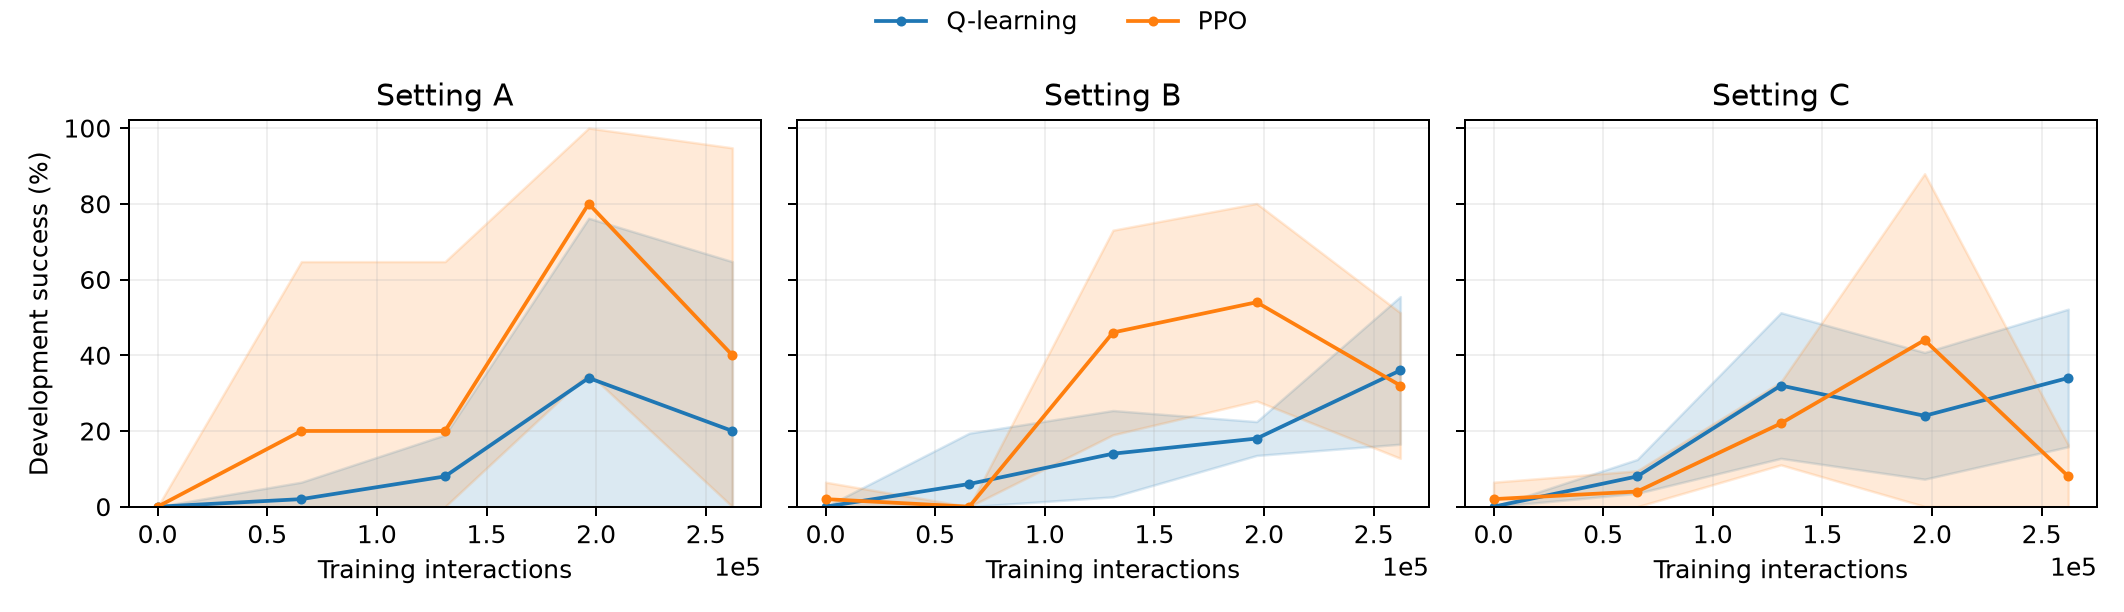
\includegraphics[width=\linewidth]{Images/part2_learning_curves_20261122.png}
\caption{Source: 22 November 2026 main experiment, training seeds 17/29/101/314/2718,
settings A/B/C and Table~\ref{tab:part2-configuration}'s configurations.
Unsmoothed mean development success, checked on ten episodes per agent at
0 and every 65,536 interactions; shading is one sample SD across five agents,
clipped to 0--100\%, not a confidence interval. Final tests are excluded.
Table~\ref{tab:part2-outcomes} evaluates development-selected checkpoints,
which can precede the curves' last point.}
\label{fig:part2-learning}
\end{figure}
